\documentclass[conference,onecolumn]{IEEEtran}
\IEEEoverridecommandlockouts
\usepackage{cite}
\usepackage{amsmath,amssymb,amsfonts}
\usepackage{algorithmic}
\usepackage{graphicx}
\usepackage{listings}
\usepackage{float}
\usepackage{textcomp}
\usepackage{gensymb}
\usepackage{xcolor}
\usepackage[spanish]{babel}
\def\BibTeX{{\rm B\kern-.05em{\sc i\kern-.025em b}\kern-.08em
    T\kern-.1667em\lower.7ex\hbox{E}\kern-.125emX}}

% --- Estilo de listados de codigo (borde verde, fondo blanco) ---
\definecolor{listinggreen}{RGB}{0,130,0}
\lstdefinestyle{tallerstyle}{backgroundcolor=\color{white},basicstyle=\ttfamily\footnotesize,breaklines=true,frame=single,rulecolor=\color{listinggreen},frameround=ffff,framesep=4pt,xleftmargin=6pt,xrightmargin=6pt,commentstyle=\color{gray},keywordstyle=\color{blue!70!black},stringstyle=\color{red!60!black},showstringspaces=false,columns=flexible,keepspaces=true,numbers=left,numberstyle=\tiny\color{gray}}
\lstset{style=tallerstyle}

\begin{document}

\title{Pr\'actica 2: Simulador de un sistema SC-FDM (DFT-spread OFDM) conforme a LTE: reducci\'on del PAPR y comparaci\'on con OFDM}

\author{\IEEEauthorblockN{Tyrone Miguel Novillo Bravo}
\IEEEauthorblockA{Facultad de Ingenier\'ia\\
Departamento de Telecomunicaciones\\
Universidad de Cuenca\\
tyrone.novillo@ucuenca.edu.ec}
\and
\IEEEauthorblockN{Freddy Eduardo L\'opez Padilla}
\IEEEauthorblockA{Facultad de Ingenier\'ia\\
Departamento de Telecomunicaciones\\
Universidad de Cuenca\\
freddy.lopez@ucuenca.edu.ec}}

\maketitle

\begin{abstract}
Este trabajo presenta la implementaci\'on y evaluaci\'on de un simulador de un sistema SC-FDM (\textit{Single-Carrier Frequency-Division Multiplexing}, tambi\'en denominado SC-FDMA), el esquema de acceso m\'ultiple del enlace ascendente de LTE. SC-FDM se construye a\~nadiendo a la cadena OFDM una precodificaci\'on por transformada discreta de Fourier (DFT-spread) de tama\~no $M$ aplicada al bloque de s\'imbolos de datos antes de la IFFT, y la transformada inversa (IDFT-despread) en el receptor; los s\'imbolos precodificados se distribuyen sobre un bloque contiguo de subportadoras (mapeo localizado). El resultado conserva las prestaciones de tasa de error de bit (BER) de OFDM pero reduce notablemente la relaci\'on de potencia pico a promedio (PAPR), lo que mejora la eficiencia del amplificador de potencia del terminal m\'ovil. El simulador reutiliza \'integramente los m\'odulos de la pr\'actica anterior (modulaciones QAM con codificaci\'on Gray, canal Pedestrian A con desvanecimiento de Rayleigh, ruido AWGN y ecualizaci\'on Zero-Forcing) y emplea las dos modulaciones del enlace ascendente: QPSK y 16-QAM. El desempe\~no se compara con OFDM mediante un an\'alisis de Monte Carlo que estima las curvas BER frente a SNR con intervalos de confianza al $95\%$ ($t$ de Student), y mediante la funci\'on de distribuci\'on acumulada complementaria (CCDF) de la PAPR, superponiendo en una sola gr\'afica las tres modulaciones de OFDM y las dos de SC-FDM. Toda la l\'ogica se implementa en Python y se expone mediante una interfaz web con pesta\~nas independientes para OFDM y SC-FDM.
\end{abstract}

\begin{IEEEkeywords}
SC-FDM, SC-FDMA, DFT-spread, PAPR, LTE, enlace ascendente, BER, Monte Carlo, OFDM, QAM.
\end{IEEEkeywords}

\section*{Objetivos}

\textbf{Objetivo general:} Implementar y evaluar un simulador de un sistema SC-FDM (DFT-spread OFDM) conforme a la numerolog\'ia de LTE, reutilizando la cadena OFDM de la pr\'actica anterior, y verificar que mantiene las mismas caracter\'isticas de BER pero con una reducci\'on significativa de la PAPR.

\textbf{Objetivos espec\'ificos:}
\begin{itemize}
    \item Implementar la precodificaci\'on DFT-spread y la decodificaci\'on IDFT-despread, junto con el mapeo localizado de subportadoras propio de SC-FDM.
    \item Integrar SC-FDM en la misma cadena de transmisi\'on, canal y recepci\'on que OFDM (canal Pedestrian A, AWGN y ecualizaci\'on Zero-Forcing), parametrizada por el esquema de acceso.
    \item Transmitir im\'agenes con las modulaciones QPSK y 16-QAM y comparar el BER de SC-FDM con el de OFDM a igualdad de SNR.
    \item Caracterizar y comparar la PAPR mediante su CCDF, superponiendo en una sola gr\'afica las tres modulaciones de OFDM y las dos de SC-FDM, y verificar la reducci\'on del PAPR de SC-FDM.
\end{itemize}

\section{Introducci\'on}

El enlace ascendente de LTE no utiliza OFDM sino su variante de portadora \'unica SC-FDMA (SC-FDM), precisamente por una limitaci\'on cr\'itica de OFDM: su elevada relaci\'on de potencia pico a promedio (PAPR). Una se\~nal OFDM es la suma coherente de cientos de subportadoras, lo que produce picos instant\'aneos muy superiores a la potencia media; estos picos obligan a operar el amplificador de potencia con un margen de retroceso (\textit{back-off}) que reduce su eficiencia. En el terminal m\'ovil, donde la energ\'ia de la bater\'ia y el costo del amplificador son cr\'iticos, esa ineficiencia es inaceptable, por lo que LTE adopta SC-FDM en el enlace ascendente \cite{myung2006scfdma,3gpp36211}.

SC-FDM conserva las ventajas de OFDM frente al multitrayecto (ecualizaci\'on sencilla por subportadora, robustez ante la interferencia entre s\'imbolos) pero a\~nade una etapa de precodificaci\'on DFT que confiere a la se\~nal transmitida un car\'acter de portadora \'unica, reduciendo as\'i su PAPR \cite{myung2008scfdma}. En este trabajo se extiende el simulador OFDM de la pr\'actica anterior para incorporar SC-FDM, reutilizando toda la cadena com\'un (modulaciones, canal Pedestrian A, AWGN y ecualizaci\'on Zero-Forcing) y a\~nadiendo \'unicamente la precodificaci\'on DFT-spread/IDFT-despread y el mapeo localizado de subportadoras. La evaluaci\'on transmite im\'agenes con QPSK y 16-QAM, compara el BER de ambos esquemas a igualdad de SNR mediante un an\'alisis de Monte Carlo con intervalos de confianza al $95\%$, y verifica la reducci\'on del PAPR de SC-FDM mediante la CCDF, todo desde una interfaz web interactiva organizada en pesta\~nas independientes.

\section{Marco te\'orico}

\subsection{SC-FDM como OFDM con precodificaci\'on DFT-spread}

SC-FDM puede entenderse como un sistema OFDM al que se a\~nade una transformada discreta de Fourier (DFT) de tama\~no $M$ que ``esparce'' (\textit{spread}) el bloque de $M$ s\'imbolos de modulaci\'on $\mathbf{d}=[d_0,\dots,d_{M-1}]$ sobre las subportadoras antes de la IFFT \cite{myung2006scfdma,cho2010mimo}. Los s\'imbolos precodificados son
\begin{equation}
D[k]=\frac{1}{\sqrt{M}}\sum_{m=0}^{M-1} d_m\, e^{-j 2\pi k m / M}, \qquad k=0,\dots,M-1, \label{eq:dftspread}
\end{equation}
y se mapean a $M$ subportadoras del s\'imbolo SC-FDM, que despu\'es se lleva al dominio temporal con la IFFT de tama\~no $N_{FFT}$ habitual de OFDM. La normalizaci\'on $1/\sqrt{M}$ es unitaria, de modo que la energ\'ia media por subportadora se conserva ($E_s=1$) y el BER resulta directamente comparable con el de OFDM. En el receptor, tras la ecualizaci\'on por subportadora, se aplica la transformada inversa (IDFT-despread) de tama\~no $M$ para recuperar los s\'imbolos de datos.

La diferencia esencial con OFDM es que en OFDM cada subportadora transporta directamente un s\'imbolo de modulaci\'on, mientras que en SC-FDM cada subportadora transporta una combinaci\'on lineal (la DFT) de todos los s\'imbolos del bloque. Por ello la se\~nal SC-FDM en el tiempo se asemeja a una transmisi\'on de portadora \'unica, con una envolvente mucho m\'as plana y, en consecuencia, una PAPR menor.

\subsection{Mapeo de subportadoras: localizado frente a distribuido}

Las $M$ salidas de la DFT pueden asignarse a las subportadoras de dos formas \cite{myung2006scfdma}: el mapeo \emph{localizado} (LFDMA), que las coloca en un bloque contiguo de subportadoras, y el mapeo \emph{distribuido} (IFDMA), que las intercala uniformemente en toda la banda. LTE emplea el mapeo localizado, que es el adoptado en este simulador. Es importante notar que la propiedad de portadora \'unica ---y por tanto la reducci\'on del PAPR--- exige que el bloque de datos ocupe subportadoras contiguas y que no se intercalen tonos piloto constantes dentro del s\'imbolo de datos; por esa raz\'on, en LTE las se\~nales de referencia de demodulaci\'on (DMRS) se transmiten en s\'imbolos SC-FDM dedicados y no mezcladas con los datos.

\subsection{PAPR y su reducci\'on en SC-FDM}

La relaci\'on de potencia pico a promedio y su funci\'on de distribuci\'on acumulada complementaria se definen como
\begin{equation}
\mathrm{PAPR}=\frac{\max_n |x[n]|^2}{\mathbb{E}[\,|x[n]|^2\,]}, \qquad \mathrm{CCDF}(\mathrm{PAPR}_0)=\Pr\{\mathrm{PAPR}>\mathrm{PAPR}_0\}.
\end{equation}
En OFDM la PAPR depende esencialmente del n\'umero de subportadoras y es pr\'acticamente independiente de la modulaci\'on \cite{han2005}. En SC-FDM, la precodificaci\'on DFT confiere a la se\~nal un comportamiento de portadora \'unica que desplaza la CCDF hacia valores menores de PAPR; la reducci\'on depende de la modulaci\'on (QPSK presenta menor PAPR que 16-QAM) y del tipo de mapeo, siendo el objetivo central de esta pr\'actica verificar dicha reducci\'on respecto a OFDM.

\subsection{Componentes reutilizados de la cadena OFDM}

El resto de la cadena es id\'entico al de la pr\'actica anterior y se reutiliza sin cambios: las modulaciones QPSK y 16-QAM con codificaci\'on Gray y energ\'ia media unitaria \cite{proakis2008digital}; el canal Pedestrian A (ITU-R M.1225) de cuatro taps con desvanecimiento de Rayleigh (Tabla~\ref{tab:pedA}) \cite{ituR1225,rappaport2002}; el ruido AWGN calibrado por SNR; la ecualizaci\'on Zero-Forcing con conocimiento perfecto del canal ($\hat{X}[k]=Y[k]/H[k]$) \cite{goldsmith2005wireless}; y la validaci\'on estad\'istica mediante Monte Carlo con intervalos de confianza basados en la distribuci\'on $t$ de Student \cite{montgomery2011}.

\begin{table}[H]
    \renewcommand{\arraystretch}{1.2}
    \caption{Perfil potencia-retardo del modelo Pedestrian A \cite{ituR1225}.}
    \label{tab:pedA}
    \centering
    \begin{tabular}{ccc}
        \hline
        \textbf{Tap} & \textbf{Retardo (ns)} & \textbf{Potencia (dB)} \\
        \hline
        1 & 0   & 0       \\
        2 & 110 & -9{,}7  \\
        3 & 190 & -19{,}2 \\
        4 & 410 & -22{,}8 \\
        \hline
    \end{tabular}
\end{table}

\section{Metodolog\'ia -- Desarrollo de la pr\'actica}

Toda la l\'ogica de procesamiento se mantiene en el m\'odulo \'unico \texttt{app.py} (Python con \texttt{numpy}, \texttt{scipy} y \texttt{Pillow}), expuesto mediante una interfaz web Flask. El c\'odigo se organiz\'o en bloques claramente segmentados para distinguir lo que es com\'un a ambas pr\'acticas de lo espec\'ifico de cada esquema: un \emph{bloque com\'un} (modulaciones QAM, c\'alculo de par\'ametros, canal, ruido, BER, PAPR de un s\'imbolo y utilidades de imagen), un \emph{bloque OFDM} (pilotos, mapeo de subportadoras e IFFT/FFT con prefijo c\'iclico), un \emph{bloque SC-FDM} (precodificaci\'on DFT-spread y mapeo localizado) y un \emph{bloque de cadena unificada} que selecciona el esquema mediante una bandera. As\'i, futuras pr\'acticas pueden reutilizar los bloques comunes sin mezclar el c\'odigo.

\subsection{Precodificaci\'on DFT-spread e IDFT-despread}

El n\'ucleo de SC-FDM son dos funciones nuevas que implementan la precodificaci\'on de \eqref{eq:dftspread} y su inversa. Ambas usan transformadas unitarias (normalizaci\'on $1/\sqrt{M}$ y $\sqrt{M}$) para preservar la energ\'ia por subportadora y garantizar que el BER de SC-FDM sea comparable al de OFDM.

\begin{lstlisting}[language=Python]
def dft_spread(bloque_datos):
    """DFT-spread unitaria de tamano M (precodificacion SC-FDM)."""
    m = len(bloque_datos)
    if m == 0:
        return bloque_datos
    return np.fft.fft(bloque_datos) / np.sqrt(m)

def idft_despread(bloque_freq):
    """IDFT-despread unitaria (inversa exacta de dft_spread)."""
    m = len(bloque_freq)
    if m == 0:
        return bloque_freq
    return np.fft.ifft(bloque_freq) * np.sqrt(m)
\end{lstlisting}

El tama\~no $M$ de la DFT coincide con el n\'umero de subportadoras de datos $N_{datos}$ del s\'imbolo. La funci\'on \texttt{dft\_spread} se aplica en el transmisor sobre el bloque de $M$ s\'imbolos QAM, y \texttt{idft\_despread} en el receptor tras la ecualizaci\'on, recuperando exactamente los s\'imbolos originales en ausencia de canal y ruido.

\subsection{Mapeo localizado de subportadoras}

La funci\'on \texttt{construir\_rejilla\_tx} es el punto exacto donde la cadena se ramifica en OFDM o SC-FDM. En OFDM coloca los s\'imbolos en las posiciones de datos e intercala pilotos cada doce subportadoras; en SC-FDM coloca el bloque DFT-spread en un \emph{bloque contiguo} de subportadoras (mapeo localizado) sin intercalar pilotos constantes, lo que preserva la propiedad de portadora \'unica y por tanto el bajo PAPR.

\begin{lstlisting}[language=Python]
def construir_rejilla_tx(bloque_datos, n_sc, n_datos, usar_dft_spread):
    if usar_dft_spread:   # --- SC-FDM: bloque contiguo localizado ---
        bloque_spread = dft_spread(np.asarray(bloque_datos, dtype=complex)[:n_datos])
        rejilla = np.zeros(n_sc, dtype=complex)
        rejilla[:len(bloque_spread)] = bloque_spread
        return rejilla
    return insertar_pilotos(bloque_datos, n_sc)   # --- OFDM: datos + pilotos ---
\end{lstlisting}

Las subportadoras no ocupadas por el bloque de datos act\'uan como banda de guarda. Esta decisi\'on de dise\~no es coherente con LTE, donde las se\~nales de referencia se transmiten en s\'imbolos dedicados; intercalar pilotos constantes dentro del s\'imbolo de datos degradar\'ia notablemente la reducci\'on del PAPR.

\subsection{Cadena unificada TX$\rightarrow$Canal$\rightarrow$RX}

La funci\'on \texttt{cadena\_tx\_rx} ejecuta el flujo completo para ambos esquemas: la bandera \texttt{usar\_dft\_spread} selecciona OFDM (\texttt{False}) o SC-FDM (\texttt{True}). El resto de la cadena ---canal Pedestrian A aplicado en frecuencia, AWGN y ecualizaci\'on Zero-Forcing--- es id\'entico al de la pr\'actica anterior.

\begin{lstlisting}[language=Python]
for i in range(n_ofdm):
    bloque_datos = simbolos_qam[i*n_datos:(i+1)*n_datos]
    rejilla = construir_rejilla_tx(bloque_datos, n_sc, n_datos, usar_dft_spread)
    senal_t, indices_fft = modulacion_ofdm(rejilla, n_fft, n_cp)
    H = generar_canal_pedestrian_a(n_fft, fs, indices_fft, rng)
    rejilla_freq = rejilla * H
    senal_canal, _ = modulacion_ofdm(rejilla_freq, n_fft, n_cp)
    senal_rx = agregar_ruido_awgn(senal_canal, snr_db, rng)
    rejilla_rx = demodulacion_ofdm(senal_rx, indices_fft, n_fft, n_cp, n_sc)
    rejilla_eq = rejilla_rx / H              # ecualizacion Zero-Forcing
    if usar_dft_spread:                      # SC-FDM: extraer bloque + IDFT-despread
        datos_rx = idft_despread(rejilla_eq[:n_datos])
    else:                                    # OFDM: posiciones de datos
        datos_rx = rejilla_eq[indices_datos_sc]
    bits_rx_total.append(mod["demapear"](datos_rx))
\end{lstlisting}

La \'unica diferencia funcional respecto a OFDM son las dos l\'ineas de la precodificaci\'on: la construcci\'on de la rejilla con \texttt{dft\_spread} en el transmisor y la \texttt{idft\_despread} sobre el bloque contiguo de datos en el receptor. La misma estrategia se aplica en la funci\'on \texttt{calcular\_papr\_ccdf}, que estima la CCDF del PAPR generando s\'imbolos aleatorios con el mapeo correspondiente a cada esquema.

\subsection{Endpoints y comparaci\'on combinada}

El \emph{endpoint} \texttt{simular} acepta un campo \texttt{esquema} (``OFDM'' o ``SC-FDM''), valida que la modulaci\'on pertenezca al esquema (SC-FDM solo admite QPSK y 16-QAM) y devuelve, adem\'as de la imagen recuperada y el BER, la comparaci\'on de la forma de onda $|x(t)|$ de OFDM y SC-FDM con los mismos datos. El \emph{endpoint} \texttt{montecarlo} acepta una lista de esquemas: con \texttt{["OFDM","SC-FDM"]} ejecuta el barrido combinado y devuelve cinco series de BER y cinco de PAPR (tres de OFDM y dos de SC-FDM) sobre un eje com\'un, listas para superponerse en una sola gr\'afica.

\subsection{Interfaz: pesta\~nas, diagrama de bloques y selecci\'on de modulaci\'on}

La interfaz se reorganiz\'o en dos pesta\~nas independientes (OFDM y SC-FDM) que comparten la misma l\'ogica mediante una factor\'ia de paneles, evitando duplicar c\'odigo. La pesta\~na SC-FDM incorpora un diagrama de bloques de la cadena (Fig.~\ref{fig:diagrama}) que resalta los bloques DFT/IDFT que la distinguen de OFDM, un mapa de cobertura con dos zonas de modulaci\'on (16-QAM cerca, QPSK en el borde, Fig.~\ref{fig:interfaz}) acorde con las dos modulaciones del enlace ascendente, y una gr\'afica de comparaci\'on de la forma de onda en el tiempo.

\begin{figure}[H]
\centering
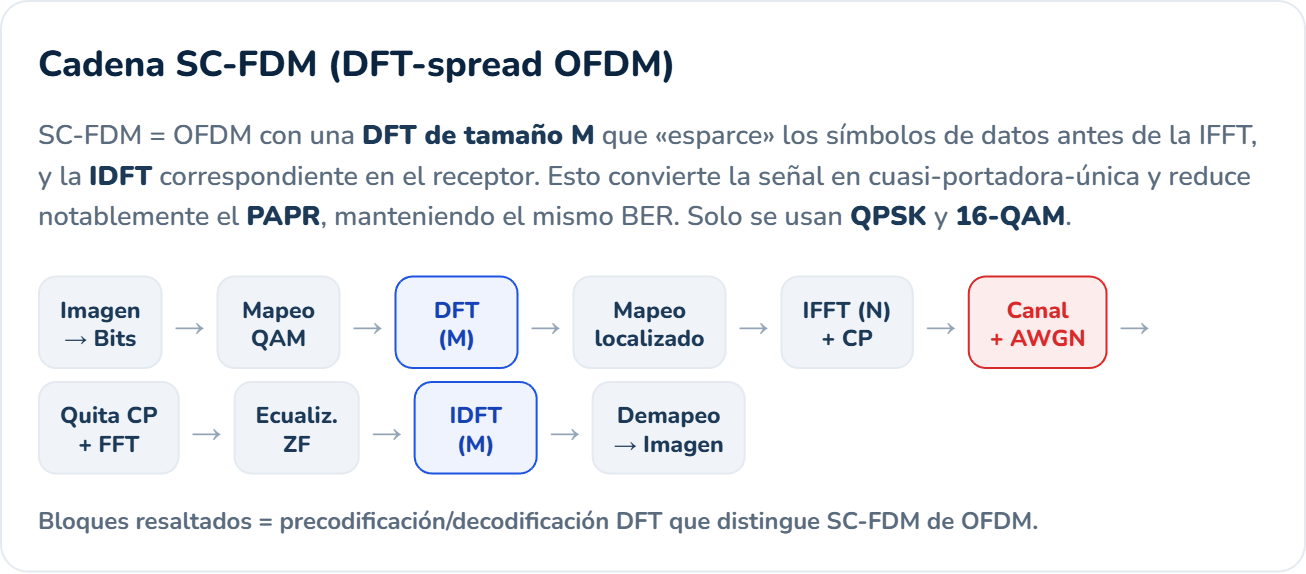
\includegraphics[width=0.95\textwidth]{img/diagrama_bloques.png}
\caption{Diagrama de bloques de la cadena SC-FDM en la interfaz; se resaltan la DFT-spread y la IDFT-despread, los bloques que la diferencian de OFDM.}
\label{fig:diagrama}
\end{figure}

\section{Evaluaci\'on -- An\'alisis de resultados}

En esta secci\'on se analizan los resultados del simulador SC-FDM. Se describe la interfaz y los par\'ametros de configuraci\'on; se examinan transmisiones de imagen con 16-QAM y QPSK; se inspeccionan la constelaci\'on recibida y el mapa de subportadoras localizado; y se comparan con OFDM la forma de onda en el tiempo, las curvas BER frente a SNR (Monte Carlo) y la CCDF de la PAPR, que constituye el resultado central de la pr\'actica.

\subsection{Interfaz y par\'ametros de configuraci\'on}

La Fig.~\ref{fig:interfaz} muestra el mapa de cobertura de la pesta\~na SC-FDM, con dos zonas asociadas a las dos modulaciones del enlace ascendente: 16-QAM en la zona interior ($0$--$600$~m) y QPSK en el borde de celda ($600$--$1500$~m). La Fig.~\ref{fig:params} resume los par\'ametros derivados para la configuraci\'on empleada ($BW{=}5$~MHz, $\Delta f{=}15$~kHz, CP normal) con una imagen de prueba de $80\times80$ p\'ixeles ($153\,600$ bits): $N_{SC}=300$ subportadoras, $N_{FFT}=512$, $f_s=7{,}680$~MHz y $N_{CP}=36$ muestras. La diferencia respecto a OFDM aparece en el tama\~no de la DFT-spread $M=275$ (igual al n\'umero de subportadoras de datos) y en el tipo de mapeo, indicado como ``Localizado (contiguo)''.

\begin{figure}[H]
\centering
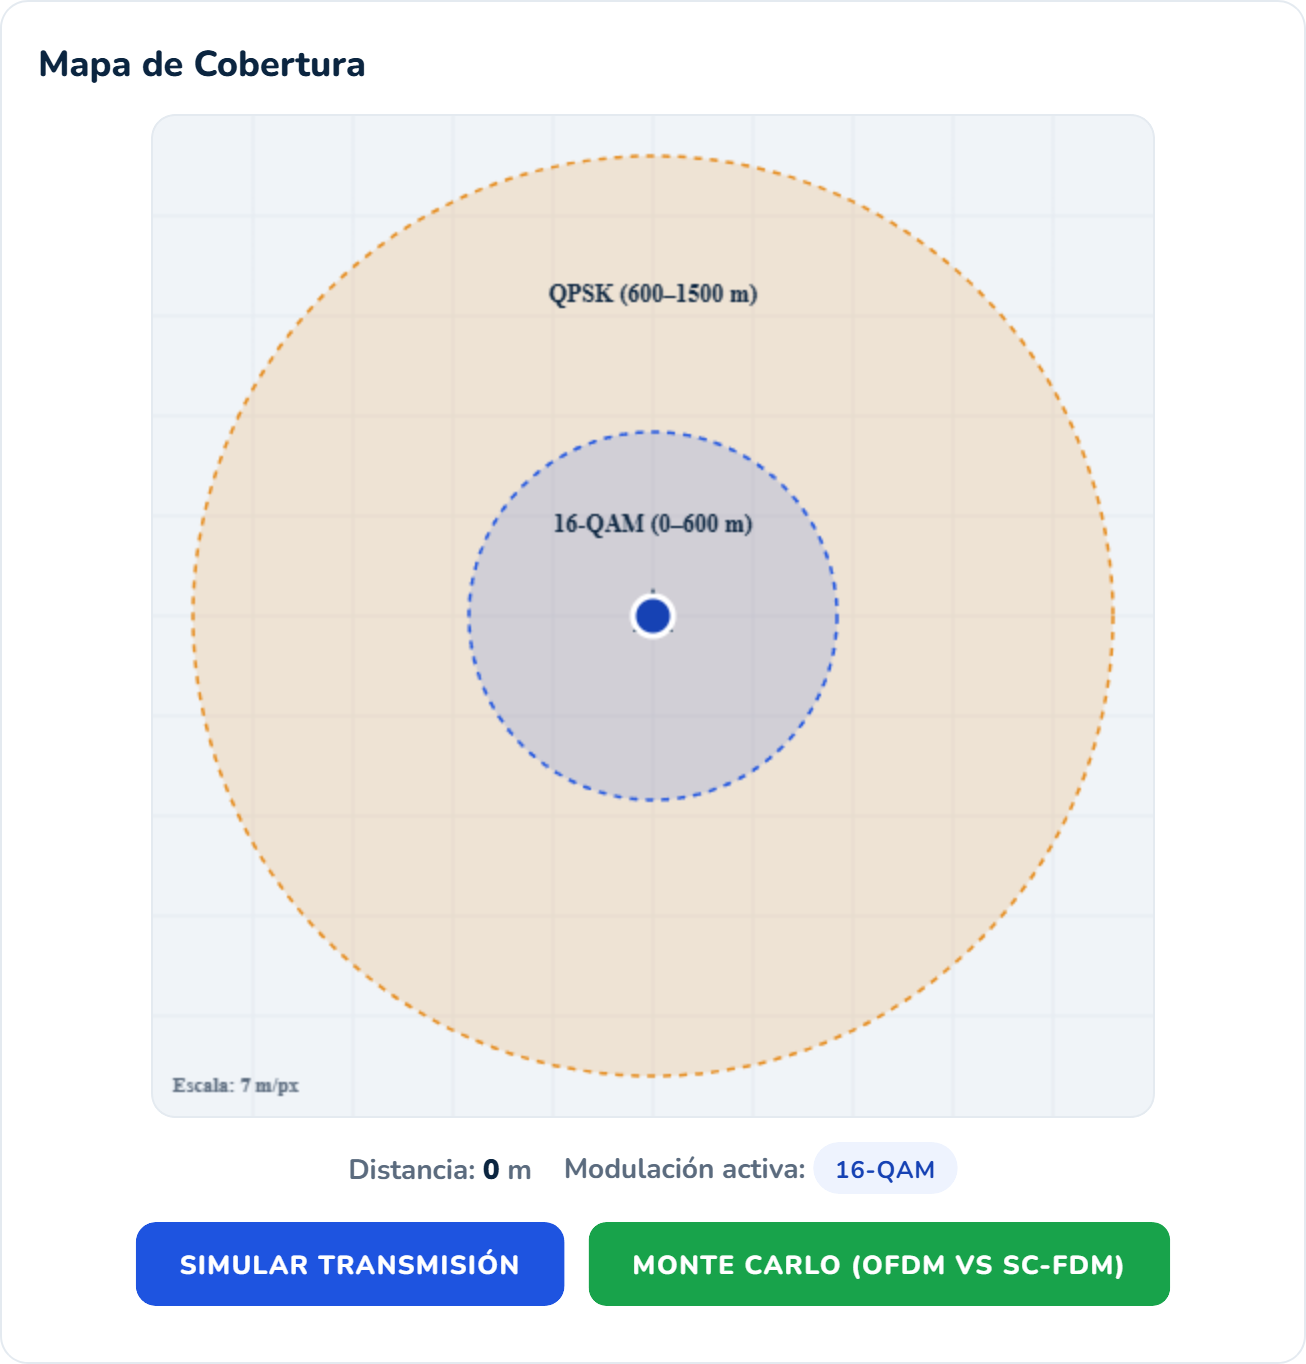
\includegraphics[width=0.7\textwidth]{img/interfaz_scfdm.png}
\caption{Mapa de cobertura de la pesta\~na SC-FDM con dos zonas de modulaci\'on: 16-QAM ($0$--$600$~m) y QPSK ($600$--$1500$~m).}
\label{fig:interfaz}
\end{figure}

\begin{figure}[H]
\centering
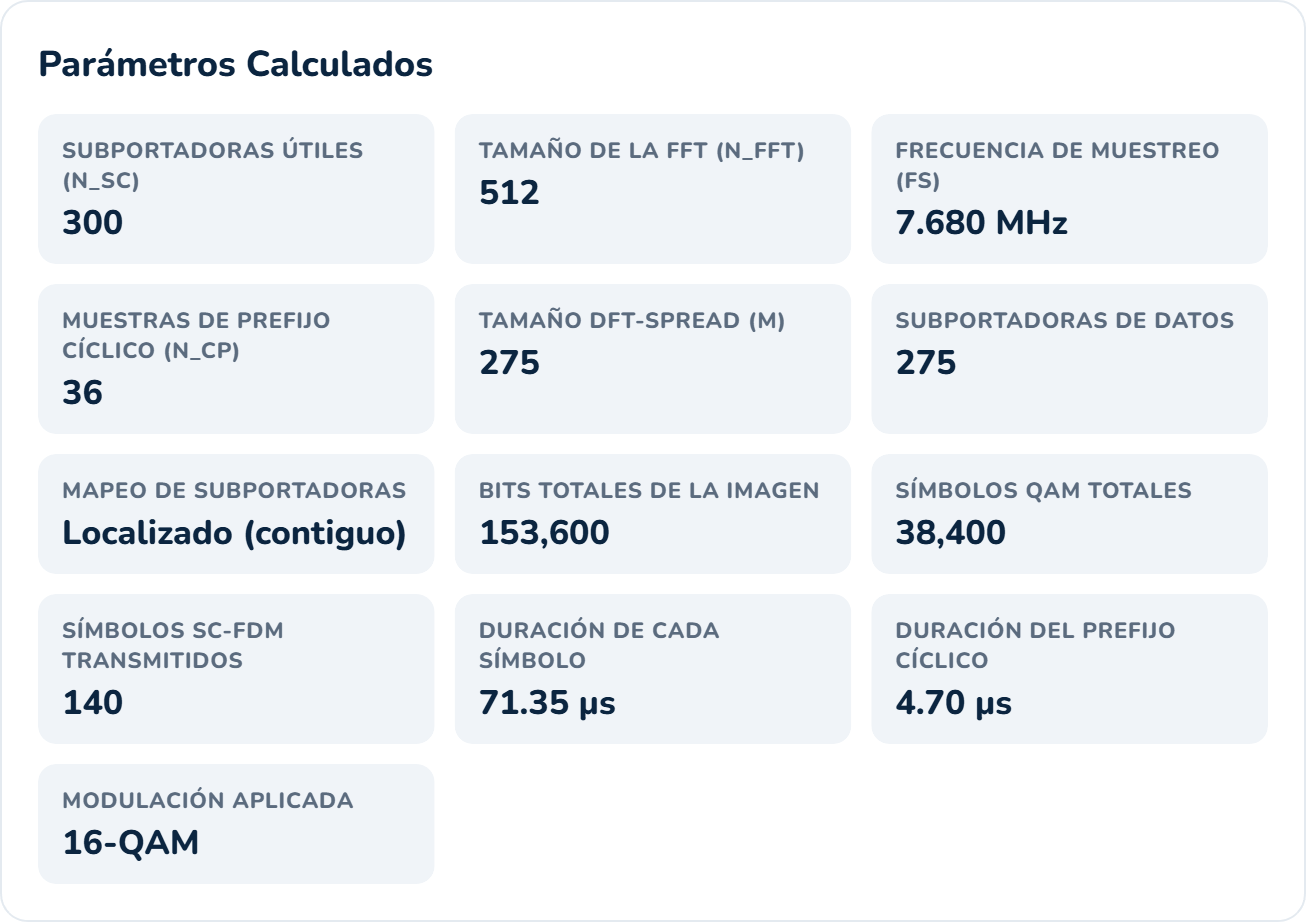
\includegraphics[width=0.95\textwidth]{img/params_scfdm.png}
\caption{Par\'ametros calculados para SC-FDM ($BW{=}5$~MHz, $\Delta f{=}15$~kHz, CP normal): $N_{SC}{=}300$, $N_{FFT}{=}512$, $M{=}275$ y mapeo localizado.}
\label{fig:params}
\end{figure}

\subsection{Transmisi\'on de im\'agenes con SC-FDM}

Se transmiti\'o la misma imagen con las dos modulaciones, resumidas en la Tabla~\ref{tab:sims}. La Fig.~\ref{fig:sim16} corresponde a 16-QAM con SNR de $25$~dB (equipo cercano a la estaci\'on base): la imagen recuperada es pr\'acticamente id\'entica a la original, con una BER de $5{,}2\times10^{-4}$. La Fig.~\ref{fig:simqpsk} corresponde a QPSK con SNR de $10$~dB a $1039$~m (borde de celda): la imagen permanece reconocible con un moteado leve y una BER de $5{,}3\times10^{-3}$, confirmando que SC-FDM hereda el comportamiento de BER de OFDM (mayor robustez de QPSK a SNR baja).

\begin{table}[H]
\centering
\caption{Resultados de las transmisiones de imagen con SC-FDM.}
\label{tab:sims}
\begin{tabular}{|l|c|c|c|c|}
\hline
\textbf{Modulaci\'on} & \textbf{SNR} & \textbf{Dist.} & \textbf{BER} & \textbf{S\'imb. SC-FDM} \\
\hline
16-QAM & $25$~dB & $0$~m    & $5{,}2\times10^{-4}$ & $140$ \\
QPSK   & $10$~dB & $1039$~m & $5{,}3\times10^{-3}$ & $280$ \\
\hline
\end{tabular}
\end{table}

\begin{figure}[H]
\centering
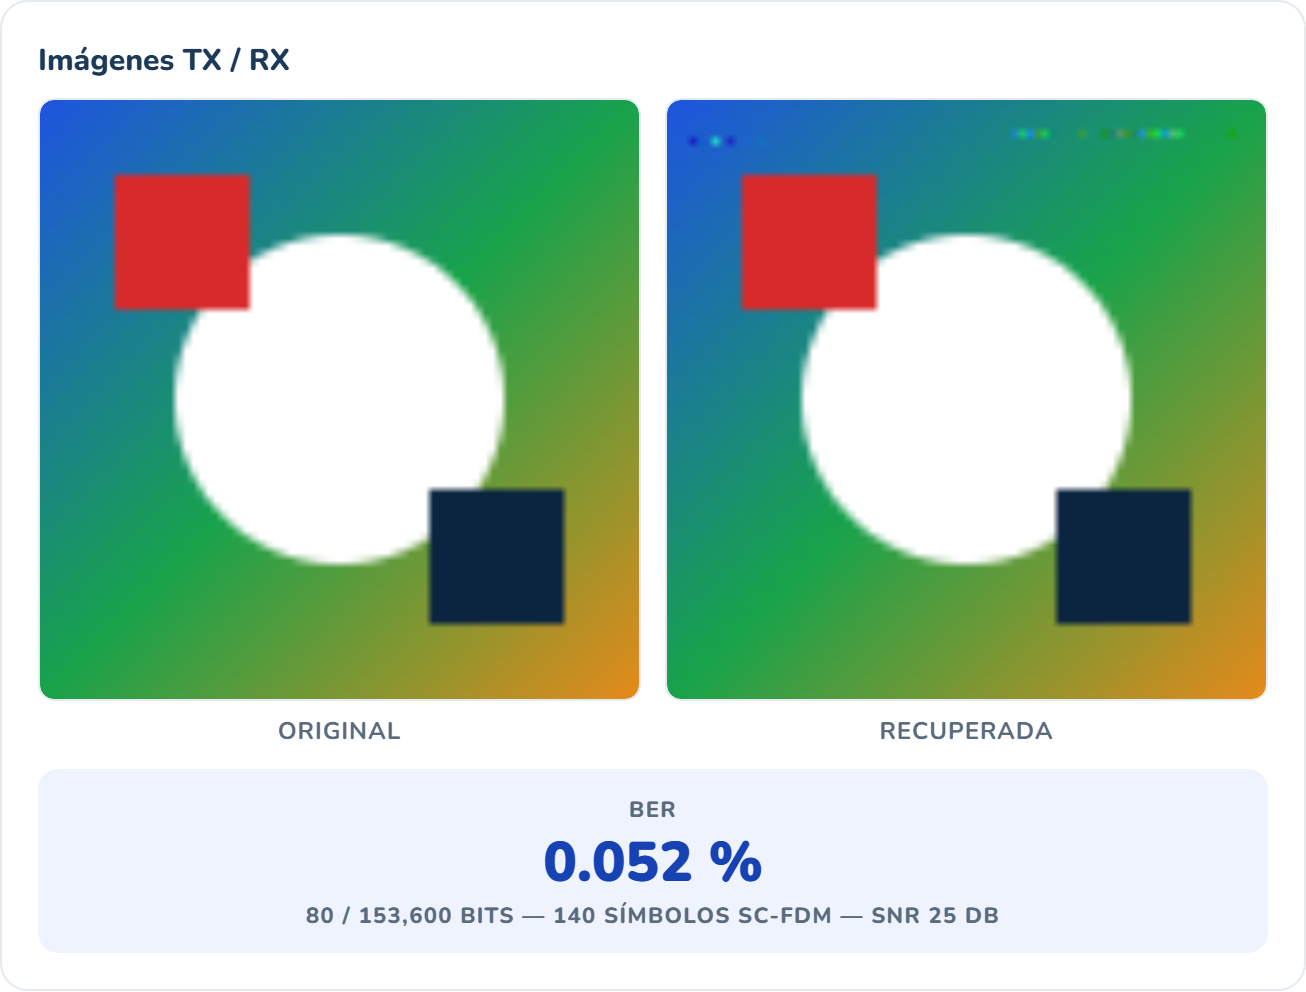
\includegraphics[width=0.6\textwidth]{img/sim_16qam_scfdm.png}
\caption{Transmisi\'on SC-FDM con 16-QAM y SNR${=}25$~dB. La imagen recuperada es pr\'acticamente id\'entica a la original (BER ${=}5{,}2\times10^{-4}$).}
\label{fig:sim16}
\end{figure}

\begin{figure}[H]
\centering
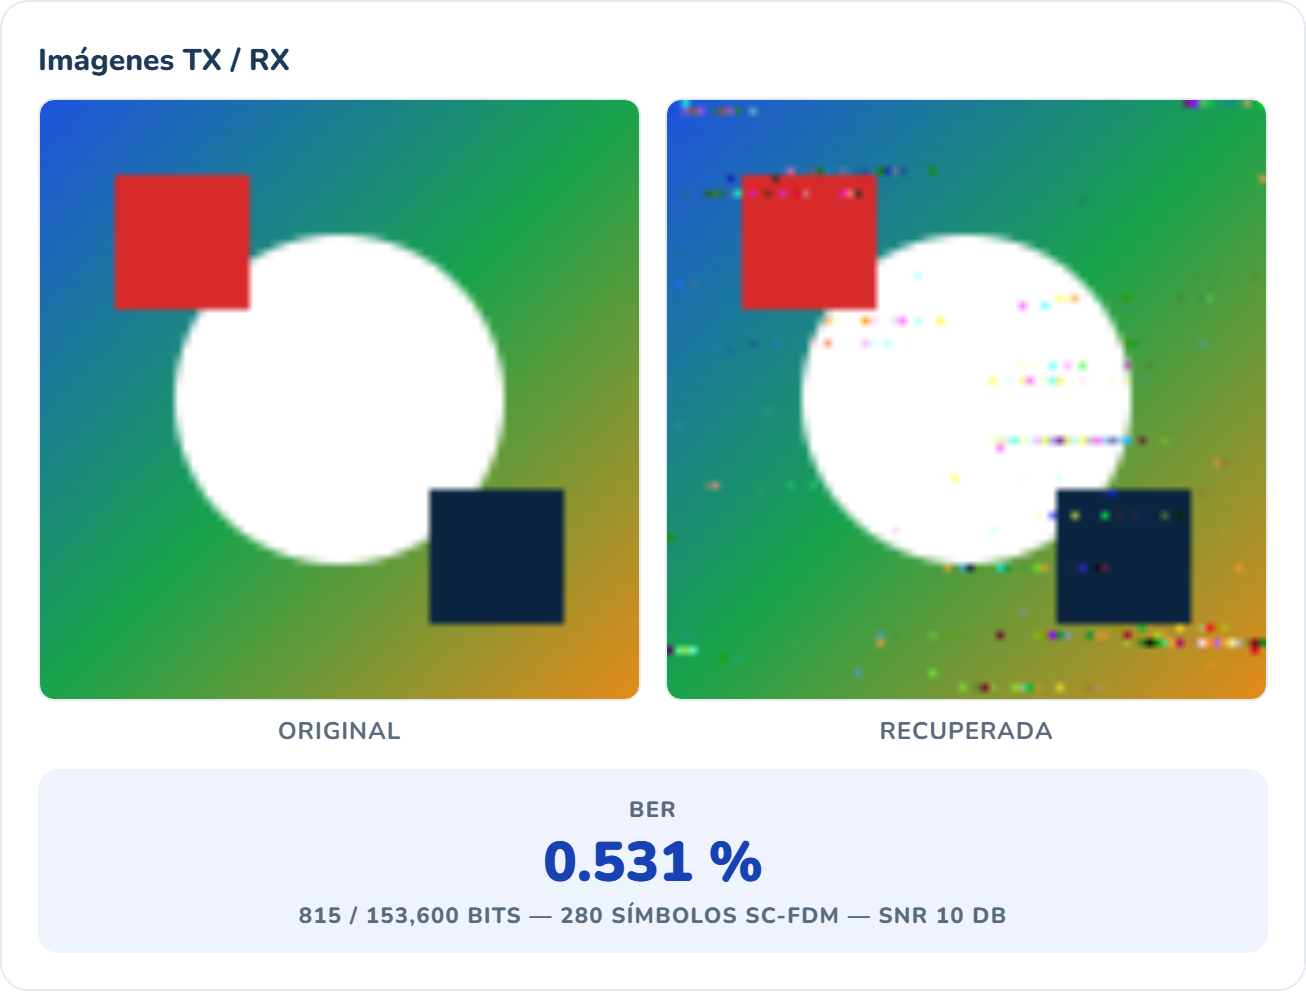
\includegraphics[width=0.6\textwidth]{img/sim_qpsk_scfdm.png}
\caption{Transmisi\'on SC-FDM con QPSK y SNR${=}10$~dB (borde de celda). La imagen sigue siendo legible (BER ${=}5{,}3\times10^{-3}$).}
\label{fig:simqpsk}
\end{figure}

\subsection{Constelaci\'on recibida y mapeo localizado de subportadoras}

La Fig.~\ref{fig:const} muestra la constelaci\'on de 16-QAM recibida tras la ecualizaci\'on Zero-Forcing y la IDFT-despread: las cruces rojas son las posiciones ideales y los puntos verdes los s\'imbolos recibidos, agrupados en torno a la ret\'icula ideal con la dispersi\'on residual debida al ruido. La Fig.~\ref{fig:mapasc} ilustra la diferencia clave del mapeo de SC-FDM frente a OFDM: en lugar de datos y pilotos intercalados, los $275$ s\'imbolos precodificados ocupan un \emph{bloque contiguo} de subportadoras (azul) y el resto act\'ua como banda de guarda (gris), sin pilotos intercalados. Es precisamente esta estructura la que preserva la propiedad de portadora \'unica y permite la reducci\'on del PAPR.

\begin{figure}[H]
\centering
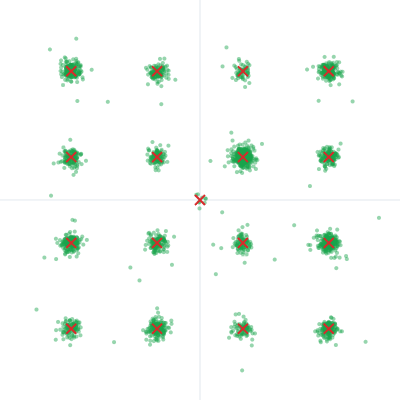
\includegraphics[width=0.5\textwidth]{img/constelacion_scfdm.png}
\caption{Constelaci\'on de 16-QAM recibida en SC-FDM tras la ecualizaci\'on Zero-Forcing y la IDFT-despread (cruces rojas: ideales; puntos verdes: recibidos).}
\label{fig:const}
\end{figure}

\begin{figure}[H]
\centering
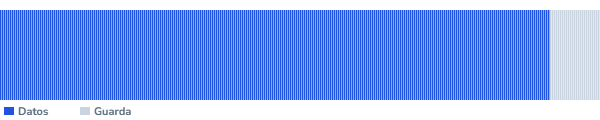
\includegraphics[width=0.95\textwidth]{img/mapa_sc_scfdm.png}
\caption{Mapa de subportadoras de SC-FDM: bloque contiguo de datos (azul) y banda de guarda (gris), sin pilotos intercalados (mapeo localizado).}
\label{fig:mapasc}
\end{figure}

\subsection{Comparaci\'on de la forma de onda en el tiempo}

La Fig.~\ref{fig:onda} compara la envolvente $|x(t)|$ de un mismo bloque de datos transmitido con OFDM y con SC-FDM. La se\~nal OFDM (rojo) presenta picos pronunciados y poco frecuentes muy por encima de su valor medio, mientras que la se\~nal SC-FDM (azul) es visiblemente m\'as plana. Para el s\'imbolo mostrado, la PAPR pasa de $9{,}93$~dB en OFDM a $5{,}97$~dB en SC-FDM, una reducci\'on cercana a $4$~dB que ilustra de forma directa la ventaja del esquema de portadora \'unica.

\begin{figure}[H]
\centering
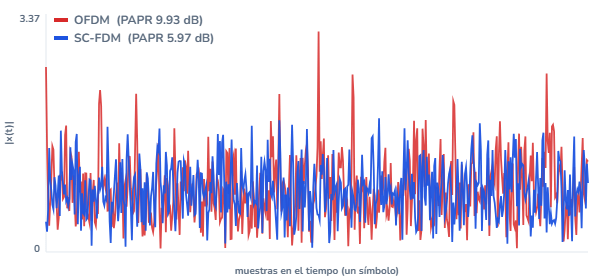
\includegraphics[width=0.9\textwidth]{img/forma_onda.png}
\caption{Envolvente $|x(t)|$ de un s\'imbolo OFDM (rojo) y SC-FDM (azul) con los mismos datos. La se\~nal SC-FDM es m\'as plana: PAPR de $9{,}93$~dB (OFDM) frente a $5{,}97$~dB (SC-FDM).}
\label{fig:onda}
\end{figure}

\subsection{Curvas BER frente a SNR (Monte Carlo)}

La Fig.~\ref{fig:montecarlo} superpone las cinco curvas de BER frente a SNR obtenidas con $10$ corridas independientes por punto e intervalos de confianza al $95\%$ ($t$ de Student): las tres modulaciones de OFDM (l\'inea continua) y las dos de SC-FDM (l\'inea discontinua), con el color identificando la modulaci\'on y las barras de error diferenciadas por estilo. Se observa que cada curva de SC-FDM sigue muy de cerca a la de OFDM de la misma modulaci\'on, confirmando el objetivo de la pr\'actica: SC-FDM mantiene las mismas caracter\'isticas de BER que OFDM. Las peque\~nas diferencias a SNR alta se deben a que la IDFT-despread promedia el ruido amplificado por la ecualizaci\'on Zero-Forcing en las subportadoras con desvanecimiento profundo, un efecto inherente al esquema de portadora \'unica.

\begin{figure}[H]
\centering
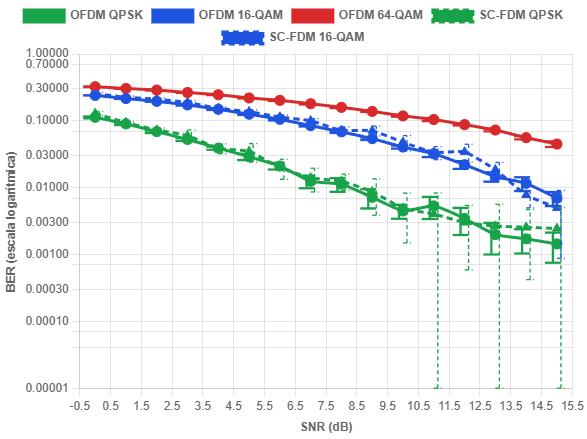
\includegraphics[width=0.9\textwidth]{img/montecarlo_comparacion.png}
\caption{BER frente a SNR: OFDM (continua, 3 modulaciones) y SC-FDM (discontinua, 2 modulaciones), Monte Carlo con $10$ corridas por punto e IC al $95\%$. Cada curva SC-FDM sigue a la de OFDM de su misma modulaci\'on.}
\label{fig:montecarlo}
\end{figure}

\subsection{CCDF de la PAPR: resultado central}

La Fig.~\ref{fig:papr} muestra la CCDF de la PAPR superponiendo las cinco curvas. Las tres de OFDM (l\'inea continua) son pr\'acticamente coincidentes y decaen hacia valores del orden de $11$--$12$~dB, confirmando que la PAPR de OFDM apenas depende de la modulaci\'on. En cambio, las dos curvas de SC-FDM (l\'inea discontinua) aparecen claramente \emph{desplazadas hacia la izquierda}: SC-FDM con QPSK alcanza el nivel de $10^{-3}$ en torno a $7{,}5$~dB y SC-FDM con 16-QAM en torno a $8{,}5$~dB, frente a los $11$--$12$~dB de OFDM. Esto representa una reducci\'on del orden de $3$ a $4$~dB en la PAPR, verificando el objetivo principal de la pr\'actica. A diferencia de OFDM, en SC-FDM la PAPR s\'i depende de la modulaci\'on (QPSK presenta menor PAPR que 16-QAM), pues la se\~nal precodificada se aproxima a una portadora \'unica cuya envolvente refleja la modulaci\'on subyacente.

\begin{figure}[H]
\centering
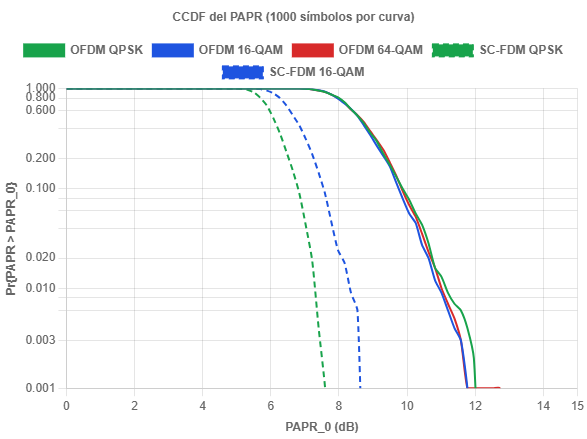
\includegraphics[width=0.9\textwidth]{img/papr_comparacion.png}
\caption{CCDF de la PAPR: OFDM (continua, 3 modulaciones) y SC-FDM (discontinua, 2 modulaciones). Las curvas de SC-FDM se desplazan a la izquierda, evidenciando la reducci\'on del PAPR ($\sim$3--4~dB).}
\label{fig:papr}
\end{figure}

\section{Conclusiones}

Se implement\'o y evalu\'o un simulador SC-FDM (DFT-spread OFDM) conforme a LTE reutilizando \'integramente la cadena OFDM de la pr\'actica anterior. La incorporaci\'on de SC-FDM requiri\'o \'unicamente dos elementos espec\'ificos ---la precodificaci\'on DFT-spread/IDFT-despread con normalizaci\'on unitaria y el mapeo localizado de subportadoras en un bloque contiguo sin pilotos intercalados---, lo que confirma que SC-FDM es, en esencia, OFDM con una etapa de precodificaci\'on adicional. La segmentaci\'on del c\'odigo en bloques comunes y espec\'ificos facilit\'o esta extensi\'on sin mezclar la l\'ogica de ambas pr\'acticas.

Los resultados verifican el doble objetivo de la pr\'actica. Por un lado, el an\'alisis de Monte Carlo mostr\'o que cada curva de BER frente a SNR de SC-FDM sigue muy de cerca a la de OFDM de la misma modulaci\'on, por lo que SC-FDM \emph{mantiene las mismas caracter\'isticas de BER}. Por otro lado, tanto la comparaci\'on de la forma de onda en el tiempo (PAPR de $9{,}93$~dB en OFDM frente a $5{,}97$~dB en SC-FDM para un mismo s\'imbolo) como la CCDF combinada del PAPR (curvas de SC-FDM desplazadas $3$--$4$~dB hacia la izquierda respecto a OFDM) evidencian una \emph{reducci\'on significativa de la PAPR}. Esta reducci\'on es precisamente la raz\'on por la que LTE adopta SC-FDM en el enlace ascendente: una menor PAPR permite operar el amplificador de potencia del terminal m\'ovil con mayor eficiencia y menor consumo, a cambio de una etapa adicional de precodificaci\'on DFT en el transmisor y el receptor.

\bibliographystyle{IEEEtran}
\bibliography{referencias}

\clearpage
\onecolumn
\newpage
\section*{Anexos}

\begin{figure}[H]
    \centering
    
\includegraphics[width=0.22\textwidth]{img/qr_sitio.png}
    \caption{C\'odigo QR del simulador desplegado: \texttt{https://ofdm.tesisucuenca.com}}
    \label{fig:qrsitio}
\end{figure}

\begin{figure}[H]
    \centering
    
\includegraphics[width=0.22\textwidth]{img/qr_repo.png}
    \caption{C\'odigo QR del repositorio del proyecto: \texttt{https://github.com/thyron001/ofdm}}
    \label{fig:qrrepo}
\end{figure}

\end{document}
